\documentclass[11pt]{report}

\usepackage[utf8]{inputenc}
\usepackage{amsmath, amsfonts, graphicx, listings, booktabs, amstext, subcaption, filecontents, csvsimple}
\usepackage[format=plain,
            textfont=it]{caption}
\usepackage[english]{babel}
\usepackage[colorinlistoftodos]{todonotes}
\usepackage[a4paper, margin=1in]{geometry}
\usepackage{url}
\usepackage{tabularx}
\usepackage{ltablex} 
\usepackage{longtable}
\usepackage{float}


\begin{document}

This is a list of mistakes, in either mathematical, grammatical/typography or explanation errors, that I feel need to be highlighted. I have made these changes in an updated copy of the paper, but following are a list of the changes that have been made.

\begin{longtable}{| p{23mm} | p{52mm}| p{70mm}|}  
\toprule
\textbf{Type of \newline modification} & \textbf{Location in paper} & \textbf{Correction} \\
\midrule[1pt]
Explanation & Abstract, 1st sentence: \newline ``used to estimate the entropy of a random vector $x \in \mathbb{R}^d$ of size $N$, based upon...'' &  ``used to estimate the entropy of a sample made up of $N$ vectors $x \in \mathbb{R}^d$, based upon...'' \\
Typography & Section 1.2.2 (pg.6), end of 1st sentence: ``aways lost'' & ``always lost'' \\
Grammatical & Section 1.2.3 (pg.9), definition of strong consistency (asymptotic normality) & Incorrect notation: Estimator $\hat{H}_{N,k}$ should be $H_{N}$ and exact entropy $H$ should be $H(f)$ \\
Explanation & Section 2.1 (pg.12), end of 1st paragraph: \newline ``asymptotic unbiasedness and consistency hold.'' & Should be more specific ``asymptotic unbiasedness and weak consistency ($\hat{H}_{N, k} \xrightarrow{p} H$) hold.'' \\
Explanation & Section 2.2.1 (pg.13), equation 2.1 & In this definition $log(\gamma)$ is the Euler-Mascheroni constant, whereas later just $\gamma$ is that constant. This caused confusion in the lines following the equation, where it should read \newline $\log (\gamma) = \log \left( \exp \left[ - \int_{0}^{\infty} e^{-t} \log(t) dt \right] \right) = - \int_{0}^{\infty} e^{-t} \log(t) dt  = -\Psi(1)$\\
Explanation & Section 2.2.1 (pg.14), 1st paragraph after equation (2.2) & When mentioning it being a consistent estimator, should be more specific as meaning weakly consistent, in that $\hat{H}_{N, k} \xrightarrow{p} H$ \\
Typography & Section 2.2 (pg.20), first line: \newline ``-L estimator''  & ``K-L estimator'' \\
Explanation & Section 2.2 (pg.20), bullet points at end of page, equations 2.20 and 2.21 & The explanation is confusing as the what $\beta$ and $a$ are, since we know $d$ and have chosen $k$ such that Theorems 1 and 2 hold, we know that $a >0.5$. So these points can be rewritten as: ``With a fixed $k$, by [5], for $a >0.5$ we have: $Bias(\hat{H}_{N, k})= O \left( \frac{1}{N^{a}} \right)$'' and ``With k depending on N, by [3], for $a >0.5$, we have: $Bias(\hat{H}_{N, k}) = O\left( \left( \frac{k}{N} \right)^{a} \right)$''\\
Typography & Chapter 3 (pg.23), number 1. in list 3rd sentence & $k \to 10$ should in fact be $k \to 11$ \\
Typography & Section 3.1 (pg.35), 3rd line after table 3.4: \newline ``since the majoring of the data'' & ``since the majority of the data'' \\
Typography & Section 3.1 (pg.37), 2nd full paragraph 3rd line: \newline ``$log(N) \approx 9$ (i.e. $N \approx 13,000$)'' & Incorrect value for $log(N)$, it should read \newline ``$log(N) \approx 9.5$ (i.e. $N \approx 13,000$)'' \\
Typography & Section 3.2 (pg.40) 2nd line: \newline ``(i.e taking a points with distance between them)'' & ``(i.e taking points with an $\infty$-small distances between them)''\\
Typography & Section 3.3.2 (pg.62) Figure 3.1.3, both graphs have been incorrectly labelled along their x-axis & Graph a) should have $2 \to 11$ not $1 \to 10$, and graph a) should also be shifted slightly. The correct graphs are shown in Figure \ref{newgraphs}\\
Mathematical & Chapter 4 (pg.71), 5th line after table 4.2: \newline ``the uniform we have variance $\frac{12}{100^2} = 0.0012$, which is significantly smaller - so we would expect a more accurate estimator due to this.'' & Formula is incorrect for variance, should be: \newline ``the uniform we have variance $\frac{100^2}{12} \approx 833$, which is much larger than the normal - however, this could be irrelevant, since there is not yet extensive research into the relationship between variance and entropy.'' \\
\hline
\end{longtable}    



\begin{figure}[H]
\makebox[\linewidth][c]{%
\begin{subfigure}[b]{.5\textwidth}
\centering
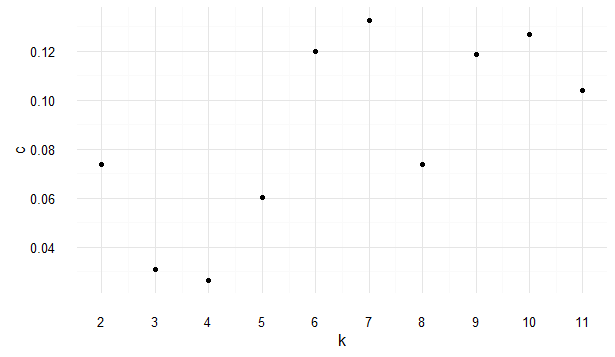
\includegraphics[width=\textwidth]{./Graphs/Best/ExpocVkFixed.png}
\caption{The values of $k$ against the values of $c_{k}$}
\end{subfigure}%
\begin{subfigure}[b]{.5\textwidth}
\centering
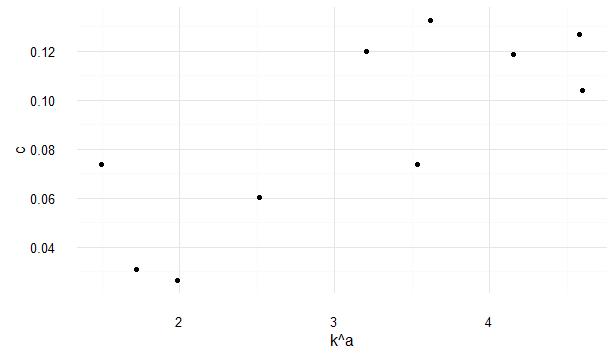
\includegraphics[width=\textwidth]{./Graphs/Best/ExpocVk2Fixed.png}
\caption{The values of $k^{a_{k}}$ against the corresponding values of $c_{k}$}
\end{subfigure}%
}
\caption{Graphically representing the relationship between $c_{k}$ and $k$ for the exponential distribution} \label{newgraphs}
\end{figure}



\end{document}